\chapter*{NSUCRYPTO 2023}
\addcontentsline{toc}{chapter}{NSUCRYPTO 2023}

\section*{Problem 1. Affine cipher}

Đây là bài 1 của round 2 và được giải bởi bạn Chương.

\subsection*{Đề bài}

Ta xét bảng chữ cái {A, ..., Z, $\alpha$, $\beta$, $\gamma$} có 29 chữ cái. Ta đánh số A, ..., Z từ 0 tới 25, và $\alpha$, $\beta$, $\gamma$ là 26, 27, 28.

Ta sử dụng cryptosystem mã hóa từng khối 2 ký tự, gọi là bigram. Với $x$ và $y$ là hai ký tự của bigram, thì plaintext sẽ là $P = 29 x + y$.

Mã hóa sử dụng biến đổi affine (giống hệ mã affine) là $C = a P + b \pmod{841}$.

Khi phân tích một đoạn văn bản dài, người ta phát hiện ra rằng các bigram sau xuất hiện nhiều nhất "$\beta\gamma$", "UM" và "LC". Đồng thời, trong tiếng Anh thì các bigram "TH", "HE" và "IN" cũng xuất hiện nhiều nhất.

\textbf{Q}. Có thể giải mã "KEUDCR" mà không cần khóa hay không? Còn key thì sao?

\subsection*{Giải}

Theo thống kê các bigram xuất hiện nhiều nhất trong ciphertext và trong plaintext sẽ khớp nhau. Do đó có thể thấy "TH" mã hóa thành "$\beta\gamma$" và "HE" mã hóa thành "LC". Như vậy ta có hệ phương trình
\begin{align*} 
    812 = a \cdot 558 + b \pmod{841} \\ 
    321 = a \cdot 207 + b \pmod{841}
\end{align*} 

Giải hệ ta có $a = 15, b = 10$. Đây là key.

Từ đây chúng ta có thể giải mã thành \textbf{CRYPTO} là plaintext ban đầu. Bài này ăn trọn 4/4 điểm.

\section*{Problem 2. Simple ideas for primes}

\subsection*{Đề bài}

Chúng ta xem xét một số dãy số bao gồm các số nguyên tố.

\begin{itemize}
    \item \textit{Số Fermat}, $F_k = 2^{2^k} + 1$, với $k$ bắt đầu từ 0. Ta có các số $F_0, F_1, F_2, F_3, F_4$ là các số nguyên tố, còn $F_5$ thì không phải.
    \item \textit{Số Mersenne}, $M_k = 2^k-1$. Ta có $M_2, M_3, M_5, M_7$ là các số nguyên tố, trong khi $M_{11}$ là hợp số. Các số nguyên tố Mersenne là các số dạng $2^k-1$ với $k$ là số nguyên tố.
    \item Dãy số $31, 331, 3\,331, 33\,331, 333\,331, 3\,333\,331, 33\,333\,331$ là các số nguyên tố được xây dựng theo quy tắc trên, nhưng số $333\,333\,331$ là hợp số chia hết cho 17.
\end{itemize}

Ta nói dãy Fermat trên có \textit{sequence primality parameter} là 5, dãy Mersenne bằng 4, dãy cuối cùng bằng 7.

\textbf{Q}. Xây dựng một dãy bao gồm các số nguyên tố như vậy. Điều kiện quan trọng ở đây là các số hạng được xác định bởi chỉ số của dãy, không phụ thuộc vào các số trước nó.

\subsection*{Giải}

Bắt đầu với dãy Euler
\begin{equation*}
    f(n) = n^2 + n + 41
\end{equation*}

Đây là dãy các số nguyên tố với $n=0, 1, \ldots, 39$ và $f(40)$ là hợp số. Như vậy đây là dãy nguyên tố độ dài 40.

Và tất nhiên, dãy "ai cũng biết" thì chỉ được 2 điểm thôi \emoji{smiling-face-with-tear}.

Sau khi tham khảo những thí sinh khác thì có một số cách xây dựng nhằm cải tiến điều này, tham khảo từ \footnote{\url{https://mathworld.wolfram.com/Prime-GeneratingPolynomial.html}}.

Nếu ta chuyển dãy trên thành
\begin{equation*}
    g(n) = f(n-40) = (n-40)^2 + (n-40) + 41 = n^2 - 79 n + 1601
\end{equation*}
thì thu được dãy số nguyên tố với độ dài 80. Các nhà toán học thế kỉ 20 đã chứng minh được rằng, nếu $p(x)$ là một đa thức sinh ra dãy số nguyên tố với $0 \leqslant x \leqslant n$ thì đa thức $p(n-x)$ cũng vậy.

Trong bảng, dãy nguyên tố có độ dài lớn nhất là 56 được biểu diễn bởi đa thức
\begin{equation*}
    \frac{1}{4} \left( n^5 - 133 n^4 + 6729 n^3 - 158379 n^2 + 1720294 n - 6823316 \right)
\end{equation*}

Dựa theo lời giải của team Himanshu Sheoran, Yo Iida và Pranshu Kumar chúng ta có thể sinh một dãy có độ dài bất kì.

Lời giải dựa trên bài blog của A. W. Walker\footnote{\url{https://awwalker.com/2017/02/27/prime-generating-polynomials/}}. Bài blog này phân tích về một bài báo năm 1977 bởi Chang và Lih với tiêu đề \emph{Polynomial Representation of Primes} nhưng hiện tại không có bản online.

Bài báo này đưa ra một phương pháp xây dựng đa thức $F(n)$ bậc $n$ mà với mọi $x \in [0, n]$ thì $F(n)$ đều là số nguyên tố.

Bài báo có thể được tóm gọn như sau. Xét đa thức
\begin{equation*}
    F(x) = 1 + \left| \sum_{n=0}^{M} \frac{a_n}{x - n} \prod_{j = 0}^{M} (x - j) \right|
\end{equation*}
sẽ sinh ra các số nguyên tố với mọi $x \in [0, M]$ nếu và chỉ nếu $a_n$ phân biệt và $(a_n \cdot M! + 1)$ là các số nguyên tố. Như vậy ta có một thuật toán đơn giản để bruteforce các đa thức trên.

\begin{algorithm}[H]
    \caption{Thuật toán sinh dãy nguyên tố độ dài $M$}
    \begin{algorithmic}
        \Require Độ dài dãy nguyên tố $M$
        \Ensure Đa thức $F(x)$ cho kết quả là số nguyên tố với mọi $x \in [0, M]$
        \State coeffs = [ ] chứa các số hạng $a_n$
        \State $an \gets 1$
        \While{Chưa đủ $M+1$ số hạng trong coeffs}
            \If{$(an \cdot M! + 1)$ là số nguyên tố}
                \State kết nạp $an$ vào dãy coeffs
            \EndIf
            \State $an \gets an + 1$
        \EndWhile
    \end{algorithmic}
\end{algorithm}


\section*{Problem 3. Mixed hashes}

\subsection*{Đề bài}

Alice và Bob trao đổi các thông điệp mã hóa. Họ dùng thuật toán mã hóa khối PRESENT với key 80-bit và ECB mode. Ở đây, thông tin được lưu dạng ảnh .ppm.

Header của file .ppm gồm 3 dòng theo dạng \textbf{P6\textbackslash nX\textbackslash nY\textbackslash n255}. Trong đó X và Y là kích thước của ảnh theo chiều ngang và dọc.

Để đảm bảo an toàn, header sẽ được loại bỏ trước khi encrypt. Để có thể khôi phục header, hash của header sẽ được gửi đi thay vì header. Khi đó 3 phần của header sẽ được ngăn cách bởi dấu cách (space) thay vì newline như trên. Nghĩa là "P6 X Y 255".

Bob chuẩn bị 8 ảnh (trong file đính kèm) mà không có header. Bob encrypt 8 ảnh đó với cùng một key theo thuật toán PRESENT và ECB mode. Bob cũng gửi hash của 8 headers đi kèm. Tuy nhiên các hash đã bị trộn lẫn với nhau. Liệu chúng ta có thể khôi phục thông điệp mà Bob muốn gửi Alice?

\subsection*{Giải}

Bài này là bài 3 ở round 1 và round 2. Trong thời gian 2 round mình đều giải ra (round 2 chi tiết hơn và trình bày đẹp hơn :v).

Đề cho một file mẫu là mikky.ppm. Khi phân tích file này mình thấy rằng, nếu gọi $w$ và $h$ là độ rộng và độ cao của ảnh (lấy từ header) thì độ dài file không có header là $3 \cdot w \cdot h$.

Sau khi encrypt bằng thuật toán mã hóa khối với ECB mode, độ dài sẽ là $3 \cdot w \cdot h + pd$, trong đó $pd$ là padding. Theo thuật toán \textbf{PRESENT} thì $0 \leqslant pd \leqslant 8$.

Với dự đoán rằng $w \approx h$, mình lấy căn bậc hai của độ dài các filel đề cho, và đưa ra dự đoán $w, h \in [400, 600]$. Nếu sai thì mình tăng độ rộng khoảng này thôi.

Tiếp theo, bruteforce $w$ và $h$ trong khoảng này, cho tới khi hash "P6 $x$ $y$ 255" xuất hiện trong số các hash trên, và \[ 0 \leqslant \text{len} (ciphertext) - 3 * w * h \leqslant 8 \] thì mình lấy $w$ và $h$ này. Thế là mình có header.

Do cả 8 file được encrypt bởi cùng một key \textbf{PRESENT}, và key có 80 bit tương ứng 10 bytes, hay 10 ký tự, nhìn đề mình nhận thấy có chuỗi \textbf{P6 X Y 255} là hợp lý. Như vậy key cho PRESENT là chuỗi \textbf{P6 X Y 255}.

Cuối cùng, mình giải mã lần lượt từng file với key trên, ghép header tương ứng vào, như vậy là mình giải mã được tất cả file rồi.

Vậy thông điệp gốc là "$\heartsuit$Loveyou". Bài này được 5/6 điểm vì không nộp code tính toán header, mất điểm vì chủ quan.

\section*{Problem 4*. Column functions}

\subsection*{Đề bài}

Alice muốn xây dựng mã đối xứng mạnh bằng việc giải một số bài toán khó.

Xét $2^n$ hàm vectorial one-to-one đôi một khác nhau, $G_i \ : \ \FF_2^n \to \FF_2^n$, với $i = 1, \ldots, 2^n$. Sử dụng các hàm này, chúng ta xây dựng một ma trận binary đặc biệt và xác định một số tính chất của nó.

Với $n=2^m$, $m \geqslant 5$, ta định nghĩa ma trận $M$ kích thước $2^n \times n 2^n$ theo quy tắc sau. Hàm thứ $i$, $i = 1, \ldots, 2^n$, là ghép của các giá trị $G_i(0, 0, \ldots, 0, 0)$, $G_i(0, 0, \ldots, 0, 1)$, \dots, $G_i(1, 1, \ldots, 1, 1)$. Các cột của $M$ có thể được xem như các vector của $n 2^n$ hàm boolean, mỗi hàm $n$ biến. Ta gọi chúng là \textit{column functions}.

Chứng minh hoặc phản bác giả thuyết sau cho ít nhất một giá trị $m \geqslant 5$: với mọi cách xây dựng ma trận như trên, tồn tại $2^{n/2}$ columns functions $f_1, \ldots, f_{2^{n/2}}$ sao cho tồn tại một hàm boolean nonzero $f: \FF_2^{2^{n/2}} \to \FF_2$ thỏa mãn các điều kiện sau:

\begin{itemize}
    \item với mọi $\bm{x} \in \FF_2^n$
    \begin{equation*}
        f(f_1(\bm{x}), f_2(\bm{x}), \ldots, f_{2^{n/2}}(\bm{x})) = 0;
    \end{equation*}
    \item với mọi $\bm{y} \in \FF_2^{2^{n/2}}$, giá trị $f(\bm{y})$ có thể tính với không quá $2^{n/2}$ phép cộng và phép nhân modulo 2.
\end{itemize}

\begin{example}
    Với $m=1$ thì $n=2$ và ta xây dựng ma trận $4 \times 8$. Xét các hàm boolean vectorial one-to-one $G_1, G_2, G_3, G_4$ từ $\FF_2^n$ tới $\FF_2^n$ xác định bởi các giá trị $(0, 1, 2, 3)$, $(0, 2, 1, 3)$, $(0, 3, 1, 2)$ và $(3, 2, 1, 0)$. Khi đó ma trận là
    \begin{equation*}
        \begin{pmatrix}
            0 & 0 & 0 & 1 & 1 & 0 & 1 & 1 \\
            0 & 0 & 1 & 0 & 0 & 1 & 1 & 1 \\
            0 & 0 & 1 & 1 & 0 & 1 & 1 & 0 \\
            1 & 1 & 1 & 0 & 0 & 1 & 0 & 0
        \end{pmatrix}
    \end{equation*}
    Ta cần tìm $2^{n/2} = 2$ column functions. Gọi $f_1$ và $f_2$ là hàm bool ứng với cột đầu và cột thứ hai của ma trận, và $f(x_1, x_2) = x_1 \oplus x_2$. Khi đó $f(f_1(\bm{x}), f_2(\bm{x})) \equiv 0$ vì $f_1(\bm{x}) = f_2(\bm{x}) = 0$ với mọi $\bm{x} \in \FF_2^n$.

    Ta cũng thấy rằng có thể chọn $f_1$ và $f_2$ là cột 5 và 6 của ma trận. Khi đó, đặt $f(x_1, x_2) = x_1 x_2$ thì $f(f_1(\bm{x}), f_2(\bm{x})) \equiv 0$ vì $f_1(\bm{x}) \neq f_2(\bm{x})$ với mọi $\bm{x} \in \FF_2^n$.

    Trong cả hai trường hợp ta chỉ cần đúng một phép tính. Lưu ý rằng hàm $f$ thỏa $f_1$ và $f_2$ được gọi là \textit{algebraically dependent}.
\end{example}

\subsection*{Giải}

Cách giải của mình không đúng hoàn toàn nên chỉ được 1/8. Dưới đây trình bày cách giải của đội Robin Jadoul, Jack Pope và Esrever Yu được 8/8 điểm.

Giả thuyết trong đề bài đúng với $m$ lớn. Ý tưởng chính là chúng ta cố định các cột sẽ chọn, có một số lượng lũy thừa các hàm $f$ (rất rất lớn) nhưng chỉ có số lượng đa thức các hàng (ít lớn hơn \emoji{rolling-on-the-floor-laughing}), do đó chúng ta có thể chọn hàm $f$ triệt tiêu tất cả hàng.

\begin{theorem}
    Cho ma trận binary $M$ kích thước $2^n \times n 2^n$. Với $n+1$ column functions bất kì, tồn tại một hàm nonzero $f: \FF_2^{n+1} \to \FF_2$ triệt tiêu trên các column functions và sử dụng nhiều nhất $2n + 1$ toán tử cộng và nhân.
\end{theorem}

\begin{proof}
    Gọi $f_1, f_2, \ldots, f_{n+1}$ là các column functions. Đặt
    \begin{equation*}
        S = \{ (f_1(\bm{x}), f_2(\bm{x}), \ldots, f_{n+1}(\bm{x})) \in \FF_2^{n+1} : \bm{x} \in \FF_2^n \}
    \end{equation*}
    là tập hợp các bộ giá trị từ các column functions. Vì $\lvert S \rvert < \lvert \FF_2^{n+1} \rvert$, ta có thể chọn vector $\bm{z} = (z_1, \ldots, z_{n+1}) \in \FF_2^{n+1} \backslash S$. Từ đây ta định nghĩa hàm $f$ là
    \begin{equation*}
        f(x_1, \ldots, x_{n+1}) = (x_1 \oplus (z_1 \oplus 1)) \cdot (x_2 \oplus (z_2 \oplus 1)) \cdots (x_{n+1} \oplus (z_{n+1} \oplus 1))
    \end{equation*}

    Lúc này, $f$ cho output là 1 chỉ khi $z$ là input (?), do đó với mọi $\bm{y} \in S$ thì $f(\bm{y}) = 0$.

    Đối với số lượng phép tính, với mọi $i$, $z_i \oplus 1$ là hằng số nên ta không xét đến khi tính số lượng phép tính cho hàm $f$. Dựa trên vector $\bm{z}$, có tối đa $n+1$ phép cộng (tương ứng $x_i \oplus (z_i \oplus 1)$) và $n$ phép nhân $n+1$ hạng tử với nhau. Vì vậy số phép tính tối đa là $2n+1$.
\end{proof}

\begin{corollary}
    Giả thuyết trên đúng với mọi $m \geqslant 4$.
\end{corollary}

\begin{proof}
    Theo định lý trên ta có $f$\footnote{Bài toán yêu cầu hàm $f$ lấy $2^{n/2}$ input. Tuy nhiên chúng ta có thể thêm các dummy input miễn là số lượng cột không lớn hơn $n+1$ (mục tiêu ban đầu)}. Bây giờ ta chỉ cần chặn lại số lượng cột mà ta cần và số lượng phép tính.

    Với số lượng cột, ta cần $n + 1 \leqslant 2^{n/2}$. Với số lượng phép tính, ta cần $2n + 1 \leqslant 2^{n/2}$. Kết hợp cả hai ta có $n \geqslant 9$, tương đương với $m \geqslant 4$.
\end{proof}

\subsection*{Bình luận}

Về tổng thể cách giải của team kia hợp lý trừ phần mình đánh dấu, chưa hiểu lắm khi $\bm{z}$ là input nghĩa là sao.

Thêm nữa, chưa có cơ sở để nghĩ ra bài giải này. Có vẻ như Esrever đã rất căng não để giải ra \emoji{smiling-face-with-tear}.

\textbf{UPDATE}. Ý nghĩa của phần đánh dấu là: trong phép tính
\begin{equation*}
    f(x_1, \ldots, x_{n+1}) = (x_1 \oplus (z_1 \oplus 1)) \cdot (x_2 \oplus (z_2 \oplus 1)) \cdots (x_{n+1} \cdot (z_{n+1} \oplus 1))
\end{equation*}

Kết quả phép tính ra 1 khi vì chỉ khi tất cả hạng tử bằng 1. Nói cách khác $x_i \oplus (z_i \oplus 1) = 1$ với mọi $1 \leqslant i \leqslant n+1$.

Điều này tương đương với $x_i = z_i$ với mọi $1 \leqslant i \leqslant n+1$. Nhưng điều này vô lý vì khi đó $\bm{x} \equiv \bm{z}$ mà hai vector này nằm ở hai tập rời nhau.

Do đó kết quả hàm $f$ luôn là 0. Ta có điều phải chứng minh.

\section*{Problem 5. Primes}

Đây là bài 5 của round 2 và được giải bởi bạn Uyên.

\subsection*{Đề bài}

Marcus chọn hai số nguyên tố lớn $p$ và $q$ rồi tính $n = p \cdot q$ và $m = p + q$. Sau đó số $n \cdot m$ được sử dụng trong cryptosystem.

Khi test Marcus thấy các số $p$ và $q$ cho tích $n \cdot m$ kết thúc bởi 2023. Điều đó khả thi không?

\subsection*{Giải}

Do $p$ và $q$ là các số nguyên tố lớn nên chúng lẻ. Suy ra $m = p + q$ là số chẵn, nên tích $n \cdot m$ cũng là số chẵn.

Số chẵn kết thúc bởi 0, 2, 4, 6, 8 nên không thể kết thúc bởi 3. Do đó điều này không thể xảy ra.

\section*{Problem 6**. An aggregated signature}

Bài này không biết làm \emoji{smiling-face-with-tear}.

\subsection*{Đề bài}

Trong một tổ chức quốc tế lớn, gọi là \textbf{NSUCRYPTO association}, mọi người quyết định tổ chức một tờ báo thông tin (news journal) trong lĩnh vực mật mã. Tổ chức muốn rằng, tin tức chỉ được công bố khi đã được kiểm duyệt bởi một nhóm lớn các nhà mật mã. Vì vậy, 10 000 chuyên gia mật mã đã được mời tới làm biên tập cho tờ báo.

Quy định công bố như sau. Tin tức được công bố khi nó được ký bởi tất cả các thành viên biên tập. Tuy nhiên các nhà mật mã không rảnh để thu thập 10 000 chữ ký cá nhân (gặp mình thì mình cũng không muốn \emoji{slightly-smiling-face}). Do đó mọi người muốn một chữ ký postquantum dùng chung mà không thể chia nhỏ ra các chữ ký cá nhân.

Yêu cầu là cần xây dựng mô hình chữ ký thỏa mãn các yêu cầu sau:

\begin{itemize}
    \item kích thước chữ ký không quá lớn, có thể hơn vài kilobytes;
    \item kích thước public key (để kiểm tra chữ ký) là nhỏ. Kích thước của key nên là cố định (hoặc gần cố định) kể cả khi số lượng chuyên gia tăng lên, ví dụ 20 000;
    \item việc kiểm tra chữ ký tốn không quá 2 phút;
    \item chữ ký có thể chống lại các tấn công trên máy tính lượng tử.
\end{itemize}

\section*{Problem 7. A unique coding}

Bài này khi nhìn đề thì "có vẻ" câu hỏi Q2 là trường hợp nhỏ hơn của Q1. Mình giải Q2 (không chắc đúng hoàn toàn) nên lời giải sau đây áp dụng cho cả Q1 và Q2.

\subsection*{Đề bài}

Xét binary error-correcting code $\mathcal{C}$ với độ dài $n$. Code này chỉ đơn giản là tập con của $\mathbb{F}_2^n$ thôi và ta truyền một phần tử của code này qua các kênh truyền.

Khi đi qua các kênh truyền các bit có thể bị sai, dẫn tới bị đảo bit. Khi nhận được vector $\bm{y} \in \mathbb{F}_2^n$, ta sẽ decode thành một phần tử thuộc $\mathcal{C}$ mà có khoảng cách gần $\bm{y}$ nhất, nói cách khác là Hamming weight ngắn nhất.

Xét cơ chế decode maximal-likelihood. Giả sử ta nhận được $\bm{y} \in \mathbb{F}_2^n$, ta muốn xét các trường hợp lỗi xảy ra ít nhất, gọi là $d_{\bm{y}}$, nghĩa là

\begin{equation*}
    d_{\bm{y}} = \min_{\bm{x} \in \mathcal{C}} wt(\bm{x}, \bm{y})
\end{equation*}

Tiếp theo, đặt $\mathcal{D} (\bm{y}) = \{ \bm{x} \in \mathcal{C} : wt(\bm{x}, \bm{y}) = d_{\bm{y}} \}$. Cuối cùng ta decode $\bm{y}$ thành phần tử $\bm{x}$ nào đó trong $\mathcal{D}(\bm{y})$.

Chúng ta quan tâm tới các trường hợp code $\mathcal{C}$ khiến $\lvert \mathcal{D}(\bm{y}) \rvert = 1$ với mọi $\bm{y} \in \mathbb{F}_2^n$. Nói cách khác khi nhận được $\bm{y}$ bất kì của $\mathbb{F}_2^n$ ta có thể decode thành một dạng duy nhất.

\textbf{Q1}. Code $\mathcal{C}$ như nào thì thỏa mãn tính chất này?

\textbf{Q2}. Code $\mathcal{C}$ như nào thỏa mãn tính chất này và là không gian tuyến tính con của $\mathbb{F}_2^n$?

\subsection*{Giải}

Đầu tiên mình có nhận xét (khá rõ ràng) sau đây:

\begin{remark}
    Với mọi $n$, code $\mathcal{C} \equiv \mathbb{F}_2^n$ thỏa mãn tính chất trên.
\end{remark}

Chúng ta có thể thấy rằng với mọi $\bm{y} \in \mathbb{F}_2^n$ nhận được thì sẽ decode thành chính nó trong $\mathcal{C}$.

Tiếp theo, ta xét nửa trên của $\mathbb{F}_2^n$. Trong hệ thập phân thì đó là các số từ $0$ tới $2^{n-1} - 1$ và có dạng \[ \bm{x} = (0, x_1, x_2, \ldots, x_{n-1}) \]

Nói cách khác, code $\mathcal{C}$ là tập hợp \[ \mathcal{C} = \{ \bm{x} = (0, x_1, x_2, \ldots, x_{n-1}): x_i \in \mathbb{F}_2 \} \]

Code $\mathcal{C}$ này thỏa mãn tính chất trên và mình sẽ chứng minh ngay sau đây.

\begin{proof}
    Giả sử ta nhận được $\bm{y} \in \mathbb{F}_2^n$. Ta có hai trường hợp:
    \begin{itemize}
        \item nếu $\bm{y} = (0, y_1, y_2, \ldots, y_{n-1})$, hay nói cách khác biểu diễn thập phân của $\bm{y}$ là từ $0$ tới $2^{n-1} - 1$, thì $\bm{y}$ được decode thành chính nó trong $\mathcal{C}$. Khi này $d_{\bm{y}} = 0$ nhỏ nhất và không có vector nào khác cho Hamming weight bằng $0$ trừ chính nó.
        \item nếu $\bm{y} = (1, y_1, y_2, \ldots, y_{n-1})$, hay nói cách khác biểu diễn thập phân của $\bm{y}$ là từ $2^{n-1}$ tới $2^n - 1$, thì $\bm{y}$ được decode thành $\bm{x} = (0, y_1, y_2, \ldots, y_{n-1})$ trong $\mathcal{C}$. Khi này $d_{\bm{y}} = 1$ nhỏ nhất vì khác mỗi bit đầu tiên và cũng không có vector nào khác cho Hamming weight bằng $1$.
    \end{itemize}
\end{proof}

Tiếp theo, mình viết các vector trong $\mathcal{C}$ thành các hàng của 1 ma trận $2^{n-1} \times n$. Gọi $A$ là ma trận hoán vị các cột của ma trận $2^{n-1} \times n$ đó. Khi đó $A$ là ma trận có tính chất: trên mỗi hàng và trên mỗi cột có đúng một phần tử (bằng 1) và ma trận $A$ khả nghịch. Ví dụ, với $n=4$, ma trận để hoán vị cột 2 với cột 4 là $\begin{pmatrix}1 & 0 & 0 & 0 \\ 0 & 0 & 0 & 1 \\ 0 & 0 & 1 & 0 \\ 0 & 1 & 0 & 0 \end{pmatrix}$.

Khi đó, nếu mình nhân ma trận $2^{n-1} \times n$ của code $\mathcal{C}$ với bất kì ma trận $A$ nào như vậy thì code $\mathcal{C}'$ nhận được cũng thỏa mãn tính chất trên.

\begin{example}
    Với $n=4$ thì code $\mathcal{C}$ gồm các vector \[ \mathcal{C} = \{ 0000, 0001, 0010, 0011, 0100, 0101, 0110, 0111 \} \]
\end{example}

Với ma trận $A$ hoán vị cột 2 và 4 như trên ta có
\begin{equation*}
    \begin{pmatrix}
        0 & 0 & 0 & 0 \\
        0 & 0 & 0 & 1 \\
        0 & 0 & 1 & 0 \\
        0 & 0 & 1 & 1 \\
        0 & 1 & 0 & 0 \\
        0 & 1 & 0 & 1 \\
        0 & 1 & 1 & 0 \\
        0 & 1 & 1 & 1 
    \end{pmatrix} \cdot 
    \begin{pmatrix}
        1 & 0 & 0 & 0 \\
        0 & 0 & 0 & 1 \\ 
        0 & 0 & 1 & 0 \\ 
        0 & 1 & 0 & 0 
    \end{pmatrix} = 
    \begin{pmatrix} 
        0 & 0 & 0 & 0 \\ 
        0 & 1 & 0 & 0 \\ 
        0 & 0 & 1 & 0 \\ 
        0 & 1 & 1 & 0 \\ 
        0 & 0 & 0 & 1 \\ 
        0 & 1 & 0 & 1 \\ 
        0 & 0 & 1 & 1 \\ 
        0 & 1 & 1 & 1
    \end{pmatrix} = \mathcal{C}'
\end{equation*}

Bây giờ mình sẽ chứng minh rằng với mọi ma trận $A$ hoán vị các cột như vậy thì code $\mathcal{C}'$ cũng thỏa mãn tính chất.

\begin{proof}  
    Đặt
    \begin{equation*}
        \mathcal{C} = \{ (0, x_1, x_2, \ldots, x_{n-1}), x_i \in \mathbb{F}_2 \}
    \end{equation*}

    Gọi $A$ là ma trận hoán vị cột kích thước $n \times n$. Khi đó ánh xạ
    \begin{equation*}
        A: \mathbb{F}_2^n \to \mathbb{F}_2^n, \quad \bm{y} \to \bm{y} \cdot A
    \end{equation*}
    là song ánh do $A$ là ma trận khả nghịch. Khi đó xét code
    \begin{equation*}\mathcal{C}' = \{ \bm{x} \cdot A: \bm{x} \in \mathcal{C} \}
    \end{equation*}

    Mình vẫn có hai trường hợp.

    \textit{Trường hợp 1.} Với $\bm{y} = (0, y_1, y_2, \ldots, y_{n-1}) \in \mathbb{F}_2^n$ từ $0$ tới $2^{n-1}-1$ như trên. Xét $\bm{y}' = \bm{y} \cdot A$.

    Khi đó, với $\bm{x} = (0, y_1, y_2, \ldots, y_{n-1}) \in \mathcal{C}$, ta có $\bm{x}' = \bm{x} \cdot A \in \mathcal{C}'$. Từ đây suy ra
    \begin{equation*}
        wt(\bm{x}' \oplus \bm{y}') = wt((\bm{x} \cdot A) \oplus (\bm{y} \cdot A)) = wt((\bm{x} \oplus \bm{y}) \cdot A) = wt(\bm{0} \cdot A) = 0
    \end{equation*}

    Ở đây $\bm{0} = (0, 0, \ldots, 0) \in \mathbb{F}_2^n$.

    Nói cách khác $d_{\bm{y}'} = 0$ và có duy nhất một vector $\bm{x}'$ được định nghĩa như trên thỏa mãn. Do đó $\lvert \mathcal{D}(\bm{y}') \rvert = 1$.

    \textit{Trường hợp 2.} Với $\bm{y} = (1, y_1, y_2, \ldots, y_{n-1}) \in \mathbb{F}_2^n$ từ $2^{n-1}$ tới $2^n-1$ như trên. Ta cũng xét $\bm{y}' = \bm{y} \cdot A$.

    Khi đó, với $\bm{x} = (0, y_1, y_2, \ldots, y_{n-1}) \in \mathcal{C}$, ta cũng có $\bm{x}' = \bm{x} \cdot \in \mathcal{C}'$. Từ đây ta có
    \begin{equation*}
        wt(\bm{x}' \oplus \bm{y}') = wt((\bm{x} \cdot A) \oplus (\bm{y} \cdot A)) = wt((\bm{x} \oplus \bm{y}) \cdot A) = wt((1, 0, 0, \ldots, 0) \cdot A) = 1
    \end{equation*}

    Ở phép nhân vector $(1, 0, \ldots, 0)$ với ma trận $A$, vì ma trận $A$ chỉ có duy nhất một cột có dạng $(1, 0, \ldots, 0)^T$ nên kết quả phép nhân là một vector có đúng một phần tử 1, còn lại là 0.

    Nói cách khác $d_{\bm{y}'} = 1$ và có duy nhất một vector $\bm{x}'$ được định nghĩa như trên thỏa mãn. Do đó $\lvert \mathcal{D}(\bm{y}') \rvert = 1$.

    Như vậy ta đã chứng minh xong.
\end{proof}

Hoàn toàn tương tự, khi code $\mathcal{C}$ là các vector bắt đầu với hai số 0 thì ta lần lượt xét $\bm{y}$ trong các khoảng $[0, 2^{n-2}-1]$, $[2^{n-2}, 2^{n-1}-1]$, $[2^{n-1}, 2^{n-1} + 2^{n-2}-1]$, $[2^{n-1} + 2^{n-2} - 1, 2^n-1]$. Nghĩa là
\begin{equation*}
    \mathcal{C} = \{ \bm{x} = (0, 0, x_1, x_2, \ldots, x_{n-2}: x_i \in \mathbb{F}_2^n) \}
\end{equation*}

Khi đó ta xét các vector $\bm{y}$ có dạng:

\begin{itemize}
    \item $\bm{y} = (0, 0, y_1, y_2, \ldots, y_{n-2})$
    \item $\bm{y} = (0, 1, y_1, y_2, \ldots, y_{n-2})$
    \item $\bm{y} = (1, 0, y_1, y_2, \ldots, y_{n-2})$
    \item $\bm{y} = (1, 1, y_1, y_2, \ldots, y_{n-2})$
\end{itemize}

Theo quy nạp thì code $C$ bắt đầu với $i$ số 0 đều đúng, $0 \leqslant i \leqslant n$. Nghĩa là
\begin{equation*}
    \mathcal{C} = \{ \bm{x} = (0, \ldots, 0, x_1, x_2, \ldots, x_{n-i}): x_i \in \mathbb{F}_2 \}
\end{equation*}

Sau đó chúng ta lại áp dụng phép nhân với ma trận hoán vị cột $A$ như bên trên thì các code $\mathcal{C}'$ cũng thỏa mãn.

Vấn đề ở đây là, những code $\mathcal{C}$ như vậy là không gian vector sinh bởi $i$ vector ($0 \leqslant i \leqslant n$) trong các vector sau:
\begin{align*}
    \bm{v}_1 & = (1, 0, 0, \ldots, 0, 0) \\ 
    \bm{v}_2 & = (0, 1, 0, \ldots, 0, 0) \\ 
    \bm{v}_3 & = (0, 0, 1, \ldots, 0, 0) \\ 
    \cdots & = \cdots \\ 
    \bm{v}_n & = (0, 0, 0, \ldots, 0, 1)
\end{align*}

Số cách chọn $i$ vector từ $n$ vector là \[ C_n^0 + C_n^1 + \ldots + C_n^n = 2^n \] cách. Nói cách khác có $2^n$ code $\mathcal{C}$ thỏa tính chất đề bài và là không gian tuyến tính của $\mathbb{F}_2^n$.

\begin{example}
    Với $n=3$ thì các code sau thỏa mãn tính chất
    \begin{align*}
        & \mathcal{C}_1 = \{ 000 \}, \\
        & \mathcal{C}_2 = \{ 000, 001 \}, \\
        & \mathcal{C}_3 = \{ 000, 010 \}, \\
        & \mathcal{C}_4 = \{ 000, 100 \}, \\
        & \mathcal{C}_5 = \{ 000, 001, 010, 011 \}, \\
        & \mathcal{C}_6 = \{ 000, 001, 100, 101 \}, \\
        & \mathcal{C}_7 = \{ 000, 010, 100, 110 \}, \\
        & \mathcal{C}_8 = \{ 000, 001, 010, 011, 100, 101, 110, 111 \}
    \end{align*}
\end{example}

\subsection*{Bình luận}

Đối với Q1 có thể thấy rằng bất cứ code nào chỉ chứa đúng một vector sẽ thỏa mãn điều kiện. Lý do là vì bất cứ $\bm{y}$ nào được gửi tới cũng sẽ decode ra vector đó.

Bài này mình được 6/12 điểm vì đưa ra cách xây dựng tốt, trình bày đẹp.

\section*{Problem 8. Algebraic cryptanalysis}

Bài này là bài 7 ở round 1 và là bài 8 ở round 2. Bài này mình giải khá qua loa ở round 1 và được giải đầy đủ, rõ ràng hơn bởi người đồng đội vip pro Chương ở round 2.

\subsection*{Đề bài}

Bob muốn xây dựng stream cipher \textbf{BOB-0.1}.

Bob sử dụng một binary key độ dài 8 là $K = (k_1, \ldots, k_8)$. Sau đó anh ấy sinh ra dãy nhị phân $\beta$ theo quy tắc:

\begin{itemize}
    \item $\beta_n = k_n$ khi $n = 1, 2, \ldots, 8$
    \item $\beta_n = \beta_{n-1} \oplus \beta_{n-8}$ khi $n \geqslant 9$
\end{itemize}

Sau đó Bob sinh dãy nhị phân $\gamma$ dùng trong phép XOR với plaintext. Dãy $\gamma$ được tạo bởi quy tắc $\gamma_n = \beta_n \cdot \beta_{n+2} \oplus \beta_{n+7}$ với $n \geqslant 1$.

Alice chặn được 8 bit của $\gamma$ sau khi để lỡ 1200 bit. Các bit đó là `00100001`. Liệu Alice có thể tìm lại được key $K$ ban đầu không?

\subsection*{Giải}

Độ dài $K$ là 8 bit, nếu chúng ta brutefore $K = (k_1, \ldots, k_8)$ rồi sinh ra 1208 bit $\gamma$ theo quy tắc trên và so sánh xem $\gamma_{1201}, \ldots, \gamma_{1208}$ nào khớp với 8 bit trên thì ta có thể biết được $K$ ban đầu là gì.

Và, bất ngờ chưa, có tới hai trường hợp $K$ thỏa mãn :v :v

Bây giờ thì chúng ta cần xem xem tại sao lại có hai trường hợp thỏa mãn.

Cùng nhau khai triển $\beta_{n+1}, \ldots, \beta_{n+8}$ theo $(\beta_{n-7}, \ldots, \beta_n)$ nào.

\begin{itemize}
    \item $\beta_{n+1} = \beta_{n} \oplus \beta_{n-7}$
    \item $\beta_{n+2} = \beta_{n+1} \oplus \beta_{n-6} = \beta_n \oplus \beta_{n-7} \oplus \beta_{n-6}$
    \item $\beta_{n+3} = \beta_{n+2} \oplus \beta_{n-5} = \beta_n \oplus \beta_{n-7} \oplus \beta_{n-6} \oplus \beta_{n-5}$
    \item $\beta_{n+4} = \beta_{n+3} \oplus \beta_{n-4} = \beta_n \oplus \beta_{n-7} \oplus \beta_{n-6} \oplus \beta_{n-5} \oplus \beta_{n-4}$
    \item $\beta_{n+5} = \beta_{n+4} \oplus \beta_{n-3} = \beta_n \oplus \beta_{n-7} \oplus \beta_{n-6} \oplus \beta_{n-5} \oplus \beta_{n-4} \oplus \beta_{n-3}$
    \item $\beta_{n+6} = \beta_{n+5} \oplus \beta_{n-2} = \beta_n \oplus \beta_{n-7} \oplus \beta_{n-6} \oplus \beta_{n-5} \oplus \beta_{n-4} \oplus \beta_{n-3} \oplus \beta_{n-2}$
    \item $\beta_{n+7} = \beta_{n+6} \oplus \beta_{n-1} = \beta_n \oplus \beta_{n-7} \oplus \beta_{n-6} \oplus \beta_{n-5} \oplus \beta_{n-4} \oplus \beta_{n-3} \oplus \beta_{n-2} \oplus \beta_{n-1}$
    \item $\beta_{n+8} = \beta_{n+7} \oplus \beta_n = \beta_{n-7} \oplus \beta_{n-6} \oplus \beta_{n-5} \oplus \beta_{n-4} \oplus \beta_{n-3} \oplus \beta_{n-2} \oplus \beta_{n-1}$
\end{itemize}

Nếu viết ở dạng phép nhân ma trận modulo 2 ta có
\begin{equation*}
    \begin{pmatrix}
        \beta_{n+1} \\ \beta_{n+2} \\ \beta_{n+3} \\ \beta_{n+4} \\ \beta_{n+5} \\ \beta_{n+6} \\ \beta_{n+7} \\ \beta_{n+8}
    \end{pmatrix} = \begin{pmatrix}
        1 & 0 & 0 & 0 & 0 & 0 & 0 & 1 \\
        1 & 1 & 0 & 0 & 0 & 0 & 0 & 1 \\
        1 & 1 & 1 & 0 & 0 & 0 & 0 & 1 \\
        1 & 1 & 1 & 1 & 0 & 0 & 0 & 1 \\
        1 & 1 & 1 & 1 & 1 & 0 & 0 & 1 \\
        1 & 1 & 1 & 1 & 1 & 1 & 0 & 1 \\
        1 & 1 & 1 & 1 & 1 & 1 & 1 & 1 \\
        1 & 1 & 1 & 1 & 1 & 1 & 1 & 0
    \end{pmatrix} \begin{pmatrix}
        \beta_{n-7} \\ \beta_{n-6} \\ \beta_{n-5} \\ \beta_{n-4} \\ \beta_{n-3} \\ \beta_{n-2} \\ \beta_{n-1} \\ \beta_n
    \end{pmatrix}
\end{equation*}

Ma trận to to kia là ma trận khả nghịch. Do đó, nếu chúng ta có các $\beta_{n+1}, \ldots, \beta_{n+8}$ thì chúng ta có thể tìm ngược lại $\beta_{n-7}, \ldots, \beta_n$. Tiếp tục quá trình này cuối cùng ta có thể tìm lại $(\beta_1, \ldots, \beta_8) = K$.

Tiếp theo, cũng tương tự, chúng ta biểu diễn dãy $\gamma$ theo $\beta$..

\begin{itemize}
    \item $\gamma_{n+1} = \beta_{n+1} \cdot \beta_{n+3} \oplus \beta_{n+8}$
    \item $\gamma_{n+2} = \beta_{n+2} \cdot \beta_{n+4} \oplus \beta_{n+1} \oplus \beta_{n+8}$
    \item $\gamma_{n+3} = \beta_{n+3} \cdot \beta_{n+5} \oplus \beta_{n+1} \oplus \beta_{n+2} \oplus \beta_{n+8}$
    \item $\gamma_{n+4} = \beta_{n+4} \cdot \beta_{n+6} \oplus \beta_{n+1} \oplus \beta_{n+2} \oplus \beta_{n+3} \oplus \beta_{n+8}$
    \item $\gamma_{n+5} = \beta_{n+5} \cdot \beta_{n+7} \oplus \beta_{n+1} \oplus \beta_{n+2} \oplus \beta_{n+3} \oplus \beta_{n+4} \oplus \beta_{n+8}$
    \item $\gamma_{n+6} = \beta_{n+6} \cdot \beta_{n+8} \oplus \beta_{n+1} \oplus \beta_{n+2} \oplus \beta_{n+3} \oplus \beta_{n+4} \oplus \beta_{n+5} \oplus \beta_{n+8}$
    \item $\gamma_{n+7} = \beta_{n+7} \cdot \beta_{n+1} \oplus \beta_{n+7} \cdot \beta_{n+8} \oplus \beta_{n+1} \oplus \beta_{n+2} \oplus \beta_{n+3} \oplus \beta_{n+4} \oplus \beta_{n+5} \oplus \beta_{n+6} \oplus \beta_{n+8}$
    \item $\gamma_{n+8} = \beta_{n+8} \cdot \beta_{n+1} \oplus \beta_{n+8} \cdot \beta_{n+2} \oplus \beta_{n+1} \oplus \beta_{n+2} \oplus \beta_{n+3} \oplus \beta_{n+4} \oplus \beta_{n+5} \oplus \beta_{n+6} \oplus \beta_{n+7}$
\end{itemize}

\textit{Trường hợp 1.} $\beta_{n+1} = 0$. Khi đó từ $\gamma_{1201}$ tới $\gamma_{1208}$ tương đương với hệ phương trình
\begin{align*}
0 & = \beta_{n+8} \\
0 & = \beta_{n+2} \cdot \beta_{n+4} \\
1 & = \beta_{n+3} \cdot \beta_{n+5} \oplus \beta_{n+2} \\
0 & = \beta_{n+4} \cdot \beta_{n+6} \oplus \beta_{n+2} \oplus \beta_{n+3} \\
0 & = \beta_{n+5} \cdot \beta_{n+7} \oplus \beta_{n+2} \oplus \beta_{n+3} \cdot \beta_{n+4} \\
0 & = \beta_{n+2} \oplus \beta_{n+3} \oplus \beta_{n+4} \oplus \beta_{n+5} \\
0 & = \beta_{n+2} \oplus \beta_{n+3} \oplus \beta_{n+4} \oplus \beta_{n+5} \oplus \beta_{n+6} \\
1 & = \beta_{n+2} \oplus \beta_{n+3} \oplus \beta_{n+4} \oplus \beta_{n+5} \oplus \beta_{n+6} \oplus \beta_{n+7} \\
\end{align*}

Hệ phương trình trên có nghiệm duy nhất $(\beta_{i}) = (0, 1, 1, 0, 0, 0, 1, 0)$.

\textit{Trường hợp 2.} $\beta_{n+1} = 1$. Tương tự hệ phương trình cũng có nghiệm duy nhất $(\beta_i) = (1, 1, 1, 0, 0, 0, 0, 1)$.

Như vậy ta có hai nghiệm thỏa mãn chuỗi 8 bit $\gamma_{1201}, \ldots, \gamma_{1208}$. Do không có điều kiện nào thêm, ta không thể xác định đâu là khóa trong hai trường hợp trên.

Bài này bạn Chương được 4/4 điểm. Good job nigga \emoji{face-with-tears-of-joy}.

\section*{Problem 9**. Finite-state machines}

Bài này không biết làm!!!

\subsection*{Đề bài}

Alice muốn tạo một generator để sinh một dãy số với độ dài chu kỳ lớn nhất có thể. Vì cô ấy biết về finite-state machine, generator $G$ sẽ được xây dựng bởi hai machine $A_1$ và $A_2$ sao cho:

\begin{itemize}
    \item $A_1 = (\FF_2^n, \FF_2, g_1, f_1)$ với hàm state-transition (hàm chuyển trạng thái) $g_1 : \FF_2^n \to \FF_2^n$ và hàm output $f_1: \FF_2^n \to \FF_2$, $n \geqslant 1$;
    \item $A_2 = (\FF_2, \FF_2^m, \FF_2, g_2, f_2)$ với hàm state-transition $g_2 : \FF_2 \times \FF_2^m \to \FF_2^n$ và hàm output $f_2 : \FF_2 \times \FF_2^m \to \FF_2$, $m \geqslant 1$.
\end{itemize}

\begin{figure}[ht]
    \centering
    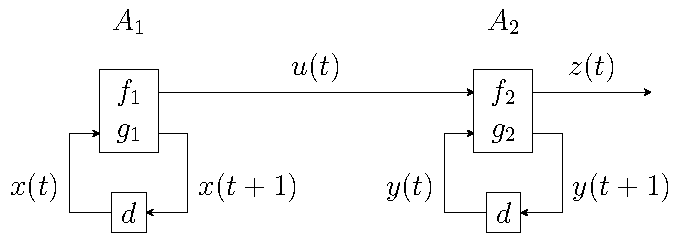
\includegraphics[page=1]{nsucrypto/2023/problem9_figures.pdf}
\end{figure}

Với mỗi $t=1, 2, \ldots$, đặt

\begin{enumerate}
    \item $x(t)$ và $y(t)$ là trạng thái của $A_1$ và $A_2$, $x(1)$ và $y(1)$ là các giá trị khởi tạo;
    \item $x(t+1) = g_1 (t)$ là trạng thái tiếp theo của $A_1$ và $u(t) = f_1 (x(t))$ là output bit của $A_1$;
    \item $y(t+1) = g_2(u(t), y(t))$ là trạng thái tiếp theo của $A_2$ và $z(t) = f_2(u(t), y(t))$ là output bit của $A_2$.
\end{enumerate}

Dãy $z(1), z(2), z(3), \ldots$ là output của generator $G$. Dễ thấy rằng dãy sinh bởi $G$ có chu kỳ nhỏ nhất không vượt quá $2^{n+m}$.

Theo thí nghiệm Alice thấy rằng, dãy output của $G$ sẽ có chu kỳ nhỏ nhất nhỏ hơn $2^{n+m}$ nếu Hamming weight của $f_1$ là chẵn. Hãy chứng minh hoặc phủ định nhận xét của Alice.

\subsection*{Giải}

Note theo gợi ý của thầy Kolomeec, chưa hiểu hết.

Dễ thấy rằng nếu $z(t)$ có chu kỳ tối đa thì các máy trạng thái $A_1$ và $A_2$ phải có chu kỳ tối đa lần lượt là $2^n$ và $2^m$.

Các giá trị của $g_2$ có thể chia ra hai phần là $g_2(0, \bm{x})$ và $g_2(1, \bm{x})$ với $\bm{x} \in \FF_2^m$. Trong đó 0 và 1 xác định từ $f_1$.

Nếu $g_2$ có chu kỳ cực đại thì trọng số phải là $2^{m}$, nói cách khác là hàm cân bằng, suy ra $g_2(0, \bm{x})$ và $g_2(1, \bm{x})$ đều có số chẵn phần tử.

Điều này có nghĩa là $g_2$ sẽ sinh ra dãy có chu kỳ tạo thành hoán vị chẵn.

Tuy nhiên nếu $g_2$ có chu kỳ cực đại thì chu kỳ đó phải tạo thành hoán vị lẻ vì khi đó hoán vị
\begin{equation*}
    1 \to 2 \to \cdots \to t \to 1 = (1, 2) (1, 3) \cdots (1, t)
\end{equation*}
có $t - 1$ tranposition. Nói cách khác đây là hoán vị lẻ vì $t=2^{m}$ chẵn.

Như vậy để chu trình đạt chu kỳ tối đa thì nó phải là hoán vị lẻ, mâu thuẫn với phân tích ở trên $g_2$ sẽ sinh ra dãy là hoán vị chẵn.

Trong cách giải này có hai chỗ mình không biết thầy lấy đâu ra: tại sao $g_2$ cân bằng thì cả $g_2(0, \bm{x})$ và $g_2(1, \bm{x})$ đều phải có số chẵn phần tử mà không phải là đều có số lẻ? Liên hệ giữa trọng số hàm bool và hoán vị chẵn/lẻ là gì?

\section*{Problem 10. Quantum encryption}

Đây là bài 8 của round 1 và bài 10 của round 2. Bài này sai gần bước cuối mới cay \emoji{loudly-crying-face}.

\subsection*{Đề bài}

Bob tạo một thuật toán mã hóa encrypt 4 bit $(x_1, x_2, x_3, x_4)$ bằng key cũng 4 bit $(k_1, k_2, k_3, k_4)$ với mạch sau:

\begin{figure}[ht]
    \centering
    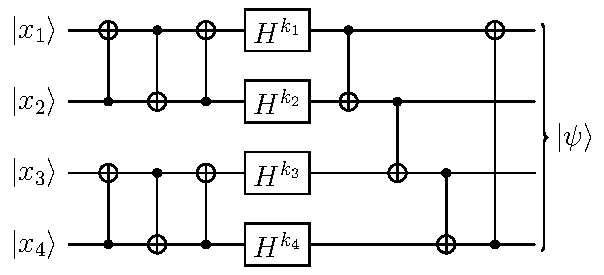
\includegraphics[page=1]{nsucrypto/2023/problem10_figures.pdf}
\end{figure}

Plaintext 4 bit $(x_1, x_2, x_3, x_4)$ được biểu diễn ở dạng 4-qubit "plainstate" $\lvert x1, x2, x3, x4 \rangle$. Quantum state này là input cho mạch ở dạng qubit đơn đi qua các cổng.

Ở đây hai loại cổng được sửa dụng là CNOT và Hadamard.

Ký hiệu $H^b$ với $b \in \{ 0, 1 \}$ có nghĩa là, nếu $b = 0$ thì cổng đồng nhất $I$ được sử dụng (không thay đổi), còn nếu $b = 1$ thì cổng Hadamard sẽ được sử dụng.

Kết quả sau khi qua mạch là "cipherstate" $\lvert \psi \rangle$.

Bob có nhiệm vụ tăng số qubit đầu vào lên nhằm giảm các sai số khi tính toán và truyền dữ liệu trên kênh quantum. Do đó Bob biến đổi thành mạch sau:

\begin{figure}[ht]
    \centering
    \includegraphics[page=2]{nsucrypto/2023/problem10_figures.pdf}
\end{figure}
Alice nói rằng cô ấy có thể tìm lại được key nếu biết $N$ amplitude của kết quả $\lvert \psi \rangle$. Do có 8 qubits ở kết quả nên số lượng amplitude tối đa là $2^8 = 256$, nói cách khác $N \leqslant 256$. Vậy Alice cần ít nhất bao nhiêu amplitude là đủ để tìm lại key?

\subsection*{Giải}

Đầu tiên xét 4 dây trên, 4 dây dưới tương tự.

\begin{figure}[ht]
    \centering
    \includegraphics[page=3]{nsucrypto/2023/problem10_figures.pdf}
\end{figure}
Chúng ta xét dây 1 và 4 của mạch (tương tự cho dây 2 và 3). Áp dụng cổng CNOT liên tiếp 3 lần ta có
\begin{equation*}
    \lvert x_1 \rangle \otimes \lvert x_2 \rangle \to \lvert x_1 \oplus x_2 \rangle \otimes \lvert x_2 \rangle \to \lvert x_1 \oplus x_2 \rangle \otimes \lvert x_1 \rangle \to \lvert x_2 \rangle \otimes \lvert x_1 \rangle
\end{equation*}

\begin{figure}[ht]
    \centering
    \begin{subfigure}{0.3\textwidth}
        \includegraphics[page=4]{nsucrypto/2023/problem10_figures.pdf}
        \caption{Dây 1 và dây 4}
    \end{subfigure}
    \begin{subfigure}{0.3\textwidth}
        \includegraphics[page=5]{nsucrypto/2023/problem10_figures.pdf}
        \caption{Dây 2 và dây 3}
    \end{subfigure}
\end{figure}

Nói cách khác là đảo bit \emoji{grinning-squinting-face}.

Tương tự cho các cặp dây (5, 8) và (6, 7). Do đó khi tới trước các cổng Hadamard thì thứ tự các qubit từ trên xuống dưới là hình \ref{nsucrypto23:p10_4}.

\begin{figure}[ht]
    \centering
    \includegraphics[page=6]{nsucrypto/2023/problem10_figures.pdf}
    \caption{Qubits trước Hadamard}
    \label{nsucrypto23:p10_4}
\end{figure}
Mạch ở dây 1 và 2 đều có dạng $\lvert x_2 \rangle$ đi qua $H^{k_1}$ nên sau khi qua cổng mình đặt $\lvert z_2 \rangle = H^{k_1} \lvert x_2 \rangle$.

Tương tự, $\lvert z_1 \rangle = H^{k_2} \lvert x_1 \rangle$ cho dây 3 và 4, $\lvert z_4 \rangle = H^{k_3} \lvert x_4 \rangle$ cho dây 5 và 6, $\lvert z_3 \rangle = H^{k_4} \lvert x_3 \rangle$ cho dây 7 và 8.

Mạch sau khi đi qua Hadamard có dạng \ref{nsucrypto23:p10_5}

\begin{figure}[ht]
    \centering
    \includegraphics[page=7]{nsucrypto/2023/problem10_figures.pdf}
    \caption{Qubits sau Hadamard}
    \label{nsucrypto23:p10_5}
\end{figure}

Ở đây chúng ta có một lưu ý nhỏ có thể giúp ích trong việc giới hạn số lượng amplitude theo đề bài. Nếu $k_1 = 0$ thì $\lvert z_2 \rangle = \lvert x_2 \rangle$. Nếu $k_1 = 1$ thì $\lvert z_2 \rangle = \dfrac{\lvert 0 \rangle + (-1)^{x_2} \lvert 1 \rangle}{\sqrt{2}}$. Như vậy, hệ số trước $\lvert 0 \rangle$ của $\lvert z_2 \rangle$ có thể là $0, 1, \dfrac{1}{\sqrt{2}}$ đều không âm.

Bây giờ chúng ta quay lại toán tử CNOT. Ma trận tương ứng của toán tử CNOT là $\begin{pmatrix} 1 & 0 & 0 & 0 \\ 0 & 1 & 0 & 0 \\ 0 & 0 & 0 & 1 \\ 0 & 0 & 1 & 0 \end{pmatrix}$. Kết quả sau khi thực hiện toán tử CNOT là hệ số trước $\lvert 00 \rangle$ và $\lvert 01 \rangle$ giữ nguyên, còn hệ số trước $\lvert 10 \rangle$ và $\lvert 11 \rangle$ đổi chỗ cho nhau.

Đối với 3 qubit, mình \textbf{dự đoán} tương tự. 

Ở cổng CNOT đầu tiên, dây 1 control dây 3. Nếu mình chỉ xét 3 dây đầu thì tích các qubit gồm $\lvert 000 \rangle$, $\lvert 001 \rangle$, $\lvert 010 \rangle$, $\lvert 011 \rangle$, $\lvert 100 \rangle$, $\lvert 101 \rangle$, $\lvert 110 \rangle$, $\lvert 111 \rangle$. 

Áp dụng "chiến thuật" tương tự, mình chỉ quan tâm vị trí 1 và 3. Nghĩa là hệ số của $\lvert 0 x 0 \rangle$ và $\lvert 0 x 1 \rangle$ giữ nguyên, còn hệ số trước $\lvert 1 x 0 \rangle$ và $\lvert 1 x 1 \rangle$ đổi chỗ cho nhau, với $x \in \{ 0, 1 \}$. Nói cách khác, 8 hệ số trước amplitude chỉ thay đổi vị trí chứ không nhiều hơn hay ít đi, hay tập hợp hệ số giữ nguyên.

\begin{figure}[ht]
    \centering
    \includegraphics[page=8]{nsucrypto/2023/problem10_figures.pdf}
\end{figure}

Như vậy, giả sử $\lvert z_2 \rangle = a \lvert 0 \rangle + b \lvert 1 \rangle$, $\lvert z_1 \rangle = c \lvert 0 \rangle + \lvert 1 \rangle$, $\lvert z_4 \rangle = e \lvert 0 \rangle + f \lvert 1 \rangle$, $\lvert z_3 \rangle = g \lvert 0 \rangle + h \lvert 1 \rangle$. Khi đó kết quả cipherstate là
\begin{equation*}
    \lvert \psi \rangle = \lvert z_2 \rangle \otimes \lvert z_2 \rangle \otimes \lvert z_1 \rangle \otimes \lvert z_1 \rangle \otimes \lvert z_4 \rangle \otimes \lvert z_4 \rangle \otimes \lvert z_3 \rangle \otimes \lvert z_3 \rangle
\end{equation*}

Xét $\lvert z_2 \rangle \otimes \lvert z_2 \rangle = a^2 \lvert 00 \rangle + ab \lvert 01 \rangle + ab \lvert 10 \rangle + b^2 \lvert 11 \rangle$. Ở đây có 3 hệ số khác nhau là $(a^2, ab, b^2)$. Với lưu ý bên trên $a \geqslant 0$ nên từ $a^2$ tính được $a$. Từ $a$, ta cần thêm $ab$ để xác định $b$.

Như vậy mình cần $2^4 = 16$ hệ số để tìm lại các key ban đầu.

\subsection*{Bình luận}

Thế éo nào mình lại nhầm khúc cuối mà lấy cả $a^2$, $ab$ và $b^2$ nên kết quả ra $3^4 = 81$. Tất nhiên là \textbf{SAI BÉT} nên chỉ được 2/8 \emoji{loudly-crying-face}.

\section*{Problem 11. AntCipher}

Bài này là bài số 2 ở round 1 và là bài số 11 ở round 2. Lúc thi round 1 mình không biết giải, còn ở round 2 thì mình đã giải theo cách như sau.

\subsection*{Đề bài}

Đặt
\begin{align*}
    f = (x_1 \lor x_2 \lor x_9) \land (\lnot x_1 \lor \lnot x_2 \lor \lnot x_9) \land (\lnot x_1 \lor x_2 \lnot x_9) \land (x_1 \lor \lnot x_2 \lor x_9) \land \\
    (x_1 \lor x_2 \lor x_3) \land (\lnot x_9 \lor \lnot x_{10} \lor \lnot x_3) \land (x_1 \lor \lnot x_2 \lor x_4) \land (\lnot x_9 \lor x_{10} \lor \lnot x_4) \land \\
    (\lnot x_1 \lor x_2 \lor x_5) \land (x_9 \lor \lnot x_{10} \lor \lnot x_5) \land (\lnot x_1 \lor \lnot x_2 \lor x_6) \land (x_9 \lor x_{10} \lor \lnot x_6) \land \\
    (x_1 \lor x_2 \lor x_3 \lor x_4 \lor \lnot x_7) \land (x_2 \lor x_3 \lor x_4 \lor \lnot x_7 \lor \lnot x_8)
\end{align*}

Hàm $f$ gồm 10 biến được viết dưới dạng CNF (conjunctive normal form). Thuật toán mã hóa dựa trên hàm $f$ biến đối hai bit plaintext $(x_1, x_2)$ thành hai bit ciphertext $(x_9, x_{10})$ khi giá trị hàm $f = True$. Hàm $f$ này có 10 biến $x_1, x_2, \ldots, x_{10}$ và 46 literals, là các hạng tử trong biểu diễn CNF của hàm. Ví dụ với dấu ngoặc thứ hai có 3 literals là $\lnot x_1$, $\lnot x_2$ và $\lnot x_9$.

\textbf{Q}. Vì các giới hạn tính toán nên chúng ta chỉ có thể sử dụng tối đa 16 biến với 20 literals. Nhắc lại rằng hàm $f$ ở trên có 10 biến và 46 literals. Hãy tìm cách biểu diễn tương đương của thuật toán mã hóa trên với giới hạn đã cho.

\subsection*{Giải}

Khi mình code hàm để tính giá trị hàm $f$ và xem xét những vector \[ \bm{x} = (x_1, \ldots, x_{10}) \] mà $f = True$, mình nhận thấy rằng:

\begin{itemize}
    \item nếu $(x_1, x_2) = (0, 0)$ thì $(x_9, x_{10}) = (1, 0)$
    \item nếu $(x_1, x_2) = (0, 1)$ thì $(x_9, x_{10}) = (1, 1)$
    \item nếu $(x_1, x_2) = (1, 0)$ thì $(x_9, x_{10}) = (0, 0)$
    \item nếu $(x_1, x_2) = (1, 1)$ thì $(x_9, x_{10}) = (0, 1)$
\end{itemize}

Mình nhận ra rằng các biến $x_3, x_4, \ldots, x_7, x_8$ hoàn toàn không tác động lên việc mã hóa từ $(x_1, x_2)$ thành $(x_9, x_{10})$ (ít nhất là ở những chỗ $f = True$ :v).

Như vậy bài toán được rút gọn thành hàm boolean 4 biến $x_1$, $x_2$, $x_9$ và $x_{10}$. Ở đó $f(0010) = f(0111) = f(1000) = f(1101) = 1$. Các vector còn lại thì $f=0$. Ở dưới là bảng chân trị \ref{nsucrypto23:prob11}.

\begin{table}[ht]
    \centering
    \begin{tabular}{|c|c|c|c|c|}
        \hline
        $x_1$ & $x_2$ & $x_9$ & $x_{10}$ & $f$ \\ \hline
        0 & 0 & 0 & 0 & 0 \\ \hline
        0 & 0 & 0 & 1 & 0 \\ \hline
        0 & 0 & 1 & 0 & 1 \\ \hline
        0 & 0 & 1 & 1 & 0 \\ \hline
        0 & 1 & 0 & 0 & 0 \\ \hline
        0 & 1 & 0 & 1 & 0 \\ \hline
        0 & 1 & 1 & 0 & 0 \\ \hline
        0 & 1 & 1 & 1 & 1 \\ \hline
        1 & 0 & 0 & 0 & 1 \\ \hline
        1 & 0 & 0 & 1 & 0 \\ \hline
        1 & 0 & 1 & 0 & 0 \\ \hline
        1 & 0 & 1 & 1 & 0 \\ \hline
        1 & 1 & 0 & 0 & 0 \\ \hline
        1 & 1 & 0 & 1 & 1 \\ \hline
        1 & 1 & 1 & 0 & 0 \\ \hline
        1 & 1 & 1 & 1 & 0 \\ \hline
    \end{tabular}
    \caption{Bảng chân trị hàm $f$}
    \label{nsucrypto23:prob11}
\end{table}

Từ bảng chân trị trên, sử dụng phương pháp bìa Karnaugh mình rút gọn được thành
\begin{align*}
    f(x_1, x_2, x_9, x_{10}) = & (\lnot x_1 \lor \lnot x_9) \land (x_1 \lor x_9) \land \\ 
    & (\lnot x_1 \lor \lnot x_2 \lor x_{10}) \land (x_1 \lor x_2 \lor \lnot x_{10}) \land \\
    & (\lnot x_1 \lor x_2 \lor \lnot x_{10}) \land (x_1 \lor \lnot x_2 \lor x_{10})
\end{align*}

CNF này có 4 biến và 16 literals, thỏa mãn yêu cầu đề bài và ăn trọn 6/6 điểm \emoji{smiling-face-with-halo}.

